\chapter{The Robot Software System (ROS)}

The ROS system is designed to contain as few customizations as possible. This allows our team and future teams to take advantage of as many pre-existing ROS packages as possible. Note that this section of the report assumes familiarity with ROS, basic ROS functionality, catkin and how to create and use ROS packages.

\section{Overview of the Packages}
The ROS software stack of the vehicle contains the following catkin packages: 

\begin{enumerate}
\item gator\textunderscore odom: Contains a script and launch file that generates the wheel odometry information
\item gator\textunderscore nav: Contains the launch and yaml files that are required to set the settings for the navigation stacks and launch the navigation stack
\item gator\textunderscore msgs: Defines any custom messages that are created specifically for the Gator
\item gator\textunderscore localization: Contains the launch files needed to launch the necessary robot\textunderscore localization and navsat\textunderscore transform nodes to allow the Gator to localize accurately
\item gator\textunderscore description: Contains the launch files, STL files and URDF file that create a visual model of the Gator
\item gator\textunderscore communication: Contains python scripts that listen to all sensor data coming from LabVIEW over UDP and publishes it in ROS to the appropriately named topic
\item gator: An unused package that was set up for the purpose of containing all the highest-level launch files for running the vehicle
\end{enumerate}

\section{Preparing to Run the ROS Stack and Setting up the Repository}

The NUC onboard the Gator already has all the packages required to run the software stack in ROS Indigo. However, if you want to run the software stack on another computer, you should try to sta with ROS Indigo unless the IV Lab has upgraded its fleet. You'll then need the following ROS packages to be isntalled using apt-get and the standard style of installing ROS packages (e.g. sudo apt-get install robot-localization-indigo):

\begin{enumerate}
\item Robot Localization: \url{http://wiki.ros.org/robot \textunderscore localization}
\item move base: \url{http://wiki.ros.org/move \textunderscore base}
\item URDF: \url{http://wiki.ros.org/urdf}
\end{enumerate}

\noindent Once these packages are installed, you can then download the Gator repository from here: \url{https://github.com/olinrobotics/GatorResearch}. Once downloaded, change directory into the master \textunderscore ws folder and then run the command "catkin \textunderscore make". Once done, run the command "source devel/setup.bash". If desired, you should add this sourcing step to your bashrc file so that you don't have to do this manually every time you open a new terminal.

\newpage

\section{ROS Navigation Overview}

The following diagram shows how the ROS Navigation Stack is designed to be used:

\begin{figure}[h!]
\centering
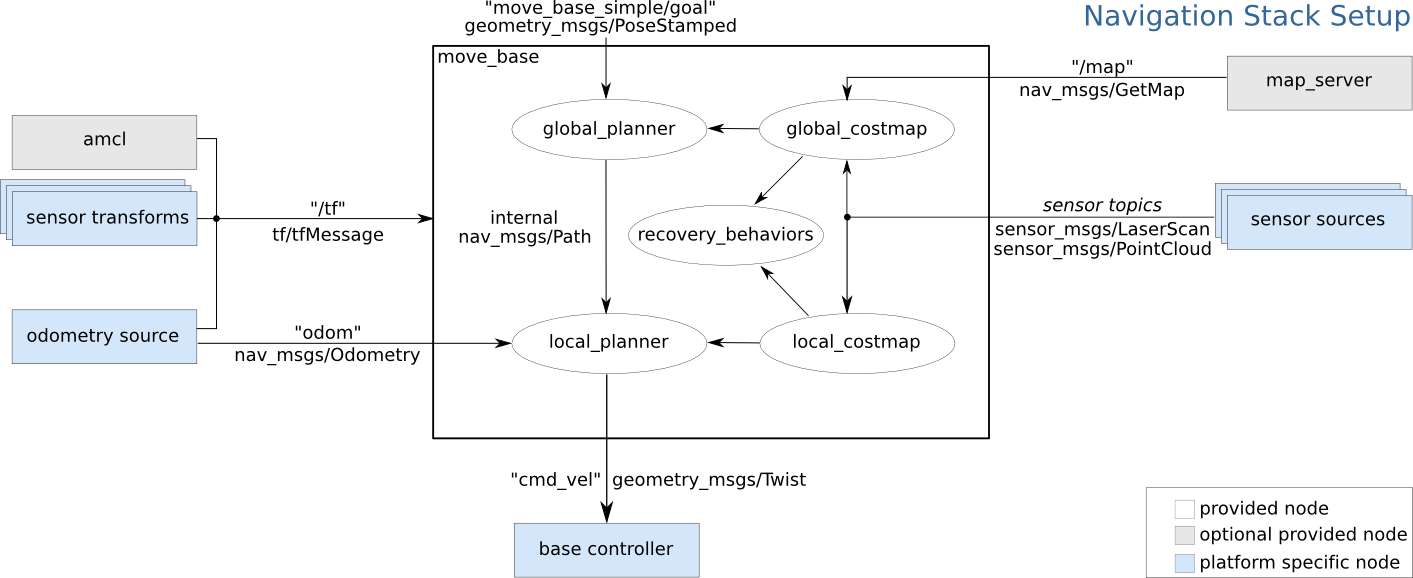
\includegraphics[scale=.35]{Photos/rosnavoverview.png}
\caption{Overview of the Setup of the ROS Navigation Stack}
\label{fig:rosnavoverview}
\end{figure} 

\section{gator\textunderscore odom}

The gator\textunderscore odom package contains the following files:

\begin{enumerate}
\item wheel\textunderscore odom.py: Creates a wheel odometry node that reads the odometry calculations made by LabVIEW and uses that odometry information to compute the odometry transform from the origin of the vehicle (i.e. on the ground under the rear axle of the vehicle) to a fixed-frame coordinate system called odom. 
\end{enumerate}
